\documentclass[10pt]{article}
\usepackage[polish]{babel}
\usepackage[utf8]{inputenc}
\usepackage[T1]{fontenc}
\usepackage{amsmath}
\usepackage{amsfonts}
\usepackage{amssymb}
\usepackage[version=4]{mhchem}
\usepackage{stmaryrd}
\usepackage{graphicx}
\usepackage[export]{adjustbox}
\graphicspath{ {./images/} }

\title{LIGA MATEMATYCZNA \\
 im. Zdzisława Matuskiego \\
 LISTOPAD 2017 \\
 SZKOEA PONADGIMNAZJALNA }

\author{}
\date{}


\begin{document}
\maketitle
\section*{ZADANIE 1.}
Trzy okręgi o promieniu \(r\), okrąg o promieniu 1 i prosta są ułożone tak, jak na rysunku. Oblicz długość promienia \(r\).\\
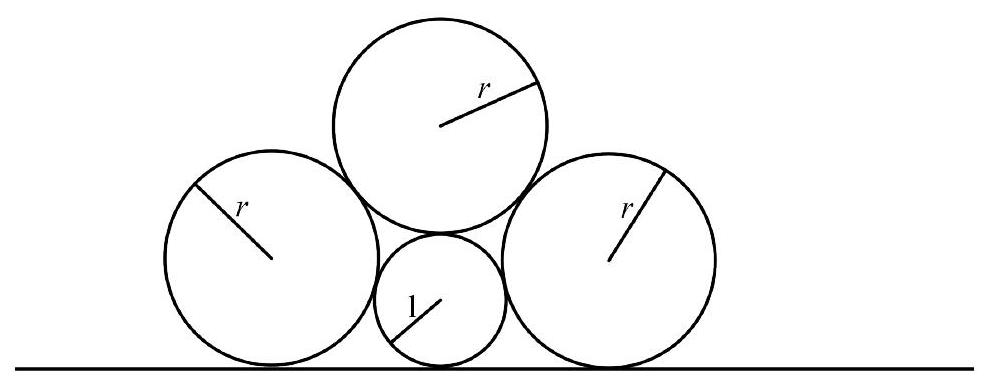
\includegraphics[max width=\textwidth, center]{2024_11_21_0fb85abfa2f5513ee193g-1}

\section*{ZADANIE 2.}
Wykaż, że liczba

\[
1^{3}+2^{3}+3^{3}+\ldots+2015^{3}+2016^{3}
\]

jest podzielna przez 2017.

\section*{ZADANIE 3.}
Znajdź wszystkie nieujemne liczby rzeczywiste \(x\) spełniające równanie

\[
[x]=\sqrt{x \cdot\{x\}}
\]

gdzie \(\{x\}=x-[x]\) oraz \([x]\) oznacza największą liczbę całkowitą nie przekraczającą liczby \(x\).

\section*{ZADANIE 4.}
Danych jest 26 kolejnych liczb naturalnych. Okazało się, że suma pewnych dziesięciu z nich jest liczbą pierwszą. Wykaż, że suma pozostałych 16 liczb jest liczbą złożoną.

\section*{ZADANIE 5.}
Wykaż, że

\[
\left(\frac{3}{2}\right)^{2016}+\left(\frac{3}{2}\right)^{2017}>\left(\frac{3}{2}\right)^{2018}
\]


\end{document}